\scanpage{124}
\[
\bigl(\|u_1\wedge\cdots\wedge u_n\|_1\bigr)^2\leq
\unsure{\surd}\alpha_n(|u_1|\wedge\mathord{-}\mathord{-}\mathord{-}\mathord{-}\wedge|u_n|)
\,\alpha_n(|u_1^+|',\cdot\mathord{-}\mathord{-}
\deleted{\unsure{\sqrt{\vphantom{u}}}}|u_n^{\deleted{\unsure{+}}}|^{\unsure{'}})
\]
\[
|\alpha_n u_1\unsure{\wedge|,}\cdot\mathord{-}u_n)|
\leq\alpha_n(|u_1|,\cdot\cdot\mathord{-}|u_n|).
\]
\begin{flushright}
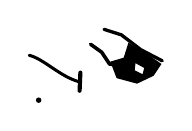
\begin{tikzpicture}[x=1cm,y=1cm,line cap=round,line join=round]
\draw[line width=1.1pt] (0,.2) .. controls (.18,.16) and (.4,-.08) .. (.65,-.14);
\draw[line width=1.5pt] (.65,-.02)--(.64,-.25);
\fill (.12,-.37) circle (.035);
\draw[line width=1.2pt] (.95,.53)--(1.17,.46)--(1.42,.27)--(1.69,.13);
\draw[line width=1.3pt] (.78,.34)--(.92,.24)--(1.02,.09)--(1.22,.06);
\fill[even odd rule] (1.03,.12)--(1.2,.17)--(1.26,.36)--(1.48,.23)--(1.68,.09)--(1.58,-.06)--(1.37,-.16)--(1.11,-.09)--cycle
 (1.35,.1)--(1.46,.04)--(1.44,-.04)--(1.34,.01)--cycle;
\end{tikzpicture}
\end{flushright}

\uline{Démonstration} \quad Posons $u_i=\sum_\alpha\lambda_\alpha^{(i)}a_\alpha^{(i)}\otimes b_\alpha^{(i)}$
(représentation canonique de $u_i$) alors
\margin{$\unsure{\mathrm I}$}
\[
|u_i|=\sum_\alpha\lambda_\alpha^{(i)}a_\alpha^{(i)},\qquad
|u_i|'=\sum_\alpha\lambda_\alpha^{(i)}b_\alpha^{(i)}
\]
\[
u_1\wedge\cdot\mathord{-}\mathord{-}\wedge u_n
=\frac{1}{n!}\sum_{\alpha_1\mathord{-}\alpha_n}
\lambda_{\alpha_1}^{(1)}\cdot\mathord{-}\lambda_{\alpha_n}^{(n)}
(a_{\alpha_1}^{(1)}\wedge\cdot\cdot\wedge a_{\alpha_n}^{(n)})
\otimes(b_{\alpha_1}^{(1)}\wedge\cdots\wedge b_{\alpha_{\unsure{n}}}^{\unsure{(n}}
\]
d'où
\[
\|u_1\wedge\cdot\mathord{-}u_n\|_1\leq\frac{1}{n!}\sum_{\alpha_1\mathord{-}\alpha_n}
\lambda_{\alpha_1}^{(1)}\mathord{-}\lambda_{\alpha_n}^{(n)}
\|a_{\alpha_1}^{(1)}\wedge\mathord{-}\wedge a_{\alpha_n}^{(n)}\|
\|b_{\alpha_1}^{(1)}\wedge\mathord{-}\wedge b_{\alpha_n}^{(n)}\|
\]
d'autre part on a, par le $=$ calcul
\[
\begin{aligned}
\alpha_n(|u_1|,\mathord{-}|u_n|)&\inserted{=\operatorname{Tr}|u_1|\wedge\mathord{-}|u_n|}=
\frac{1}{n!}\sum_{\alpha_1\mathord{-}\alpha_n}\lambda_{\alpha_1}^{(1)}\mathord{-}\lambda_{\alpha_n}^{(n)}
\|a_{\alpha_1}^{(1)}\wedge\mathord{-}a_{\alpha_n}^{(n)}\|^2
\deleted{\unsure{b_{\alpha_1}^{(1)}\wedge\ldots\wedge a_{\alpha_n}^{(n)}}}\\
\alpha_n(|u_1|',\cdot\mathord{-}|u_n|')&=\frac{1}{n!}\sum_{\alpha_1\mathord{-}\alpha_n}
\lambda_{\alpha_1}^{(1)}\mathord{-}\lambda_{\alpha_n}^{(n)}
\|b_{\alpha_1}^{1}\wedge\mathord{-}\wedge b_{\alpha_n}^{(n)}\|^2
\end{aligned}
\]
\margin{$\unsure{\lambda|\alpha}_n=$}
L'inégalité voulue \deleted{\unsure{est}} \unsure{:|est} alors conséquence de l'inégalité
\[
\deleted{\unsure{(a_{\alpha_1}^{(1)}\wedge\ldots\wedge a_{\alpha_n}^{(n)},b_{\alpha_1}^{(1)}\wedge\ldots\wedge b_{\alpha_n}^{(n)})}}
\]
\margin{$\unsure{\mathrm{II}}$}
de Cauchy-Schwartz.

\par\medskip\noindent
\hbox{\rlap{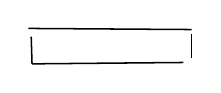
\begin{tikzpicture}[baseline=0pt,x=1em,y=1em,line width=.55pt]
\draw (-.1,1)--(5.8,.96);
\draw (0,.7)--(.03,-.28);
\draw (.03,-.28)--(5.5,-.23);
\draw (5.8,.81)--(5.8,-.06);
\end{tikzpicture}}\kern.25em Corollaire 1\kern.45em}
\[
|\alpha_n\unsure{(}u_1,\mathord{-}u_n)|\leq\|u_1\wedge\mathord{-}\wedge u_n\|_1
\leq\frac{1}{2}\bigl(\alpha_n(|u_1|,\cdot\mathord{-}|u_n|)+\alpha_n(|u_1|',\mathord{-}\mathord{-}|u_n|')\bigr)
\]

\par\medskip\noindent
\hbox{\rlap{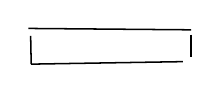
\begin{tikzpicture}[baseline=0pt,x=1em,y=1em,line width=.55pt]
\draw (-.08,1)--(5.8,.95);
\draw (0,.73)--(.02,-.29);
\draw (.02,-.29)--(5.5,-.2);
\draw (5.8,.78)--(5.8,-.04);
\end{tikzpicture}}\kern.25em Corollaire 2\kern.45em}
\[
|\alpha_n(A+B)|^2\leq\deleted{\unsure{\sqrt{\vphantom A}}}\alpha_n(|A|+|B|)
\alpha_n(|A^{\unsure{*}}|'+|B^{\unsure{*}}|^{\unsure{+|'}})
\]
En effet, on a \deleted{\unsure{$\alpha_n(A+B$}}
\[
\begin{aligned}
|\alpha_n(A+B)|^{\unsure{2}}&=\left|\sum_k C_k^n\alpha_n(\overbrace{A,\mathord{-}A}^{k},
\overbrace{B,\mathord{-}B}^{n-k})\right|^{\unsure{2}}\\
&\leq\deleted{\unsure{\surd}}\sum_k C_k^n
\bigl(\alpha_n(\overbrace{|A|,\mathord{-}\unsure{A|\lvert A}}^{k},\overbrace{\unsure{\lvert A\rvert|\lvert B\rvert},\mathord{-}\unsure{B_1|B,|\lvert B\rvert}}^{n-k})\bigr)^{1/2}
\bigl(\sum_k\alpha_n(\overbrace{|A|',\mathord{-}|A|'}^{k},|B|'\mathord{-}\mathord{-})\bigr)^{1/2}
\end{aligned}
\]
\margin{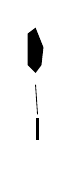
\begin{tikzpicture}[x=.025cm,y=-.025cm]
\fill (0,0)--(4,-3)--(8,7)--(7,16)--(4,20)--(0,16)--cycle;
\draw[line width=.3pt] (4,26)--(5,41);
\draw[line width=.8pt] (5,43)--(5,54);
\end{tikzpicture}}
d'où, par l'inégalité de Cauchy-Schwartz
\[
|\alpha_n(A+B)|^{\unsure{2}}\leq\bigl(\sum_k C_k^n\alpha_n
\unsure{\lvert A\rvert,\mathord{-}\lvert A\rvert,\lvert B\rvert\mathord{-}B,)|
(\lvert A\rvert,\mathord{-}\lvert A\rvert,\lvert B\rvert\mathord{-}B,)}\bigr)^{1/2}
\bigl(\sum_k{}'\quad\bigr)^{\unsure{1/2}}\unsure{!}
\]
\margin{125}
